\documentclass[12pt]{article}

\usepackage{graphicx,amsmath,textcomp,caption,subcaption,url}
\usepackage[round]{natbib}
\usepackage[margin=2cm]{geometry}
%\usepackage[subtle]{savetrees}
\linespread{1.1}
\bibliographystyle{plainnat}
\title{
ENGN1218 Introduction to Electronics\\
Full-wave Rectifier Analysis\\
}
\author{
\and Paul Apelt, u5568225
\and Thomas Hale, u5567957
\and School of Engineering, ANU 
}
\begin{document}
\maketitle

\begin{abstract}
A diode-bridge full wave power rectifier circuit was designed and constructed. The aim was to achieve a 12V DC output with 10\% tolerance. A theoretical analysis of two types of diode-bridge full-wave rectifiers---with and without a capacitor---was conducted, and results confirmed using a computer simulation. The construction process was documented, and all output parameters measured. The aim was successfully achieved, with all output parameters matching the predicted values within an acceptable error bound.
\end{abstract}

\section{Introduction}
\label{sec:int}
Most forms of power are supplied in the form of AC current. As most electronics devices and systems require DC current it is necessary that there be a means to convert AC to DC. Power rectifier circuits allow this and function using diodes, which ideally only allow the passage of current in one direction---typically the positive direction.

There are several types of rectifier circuits that can be used to convert from AC to DC current but only the full wave rectifier or bridge rectifier will be discussed in this report. The bridge rectifier circuit---as per Figure~\ref{fig:cap}---is designed such that current during both the negative and positive cycles pass through the load site in the same direction, which means that the voltage across the load site is always of the same sign. Although this configuration of diodes succeeds in inverting the voltage in the negative cycle, the voltage is not the constant DC voltage that is desired. In order to reduce this voltage variation a capacitor is added in series with the load site. The capacitor charges when the voltage from the source is increasing and discharges when the voltage from the source is decreasing, thus smoothing the output waveform. 

The analysis of the full-wave rectifier was conducted using multiple techniques, which are detailed in the body of the report. In the theoretical analysis several equations were used to approximate the output and ripple voltages of the voltage across the load resistor in the circuit. These same values were then calculated using a PSPICE simulation. The simulation was also used to observe the effect of various diode malfunctions on the function of the rectifier circuit. In the implementation section, the method used to construct the physical rectifier is described and how the output and ripple voltages of the load resistor were measured. Photos of the soldered and functioning circuit are also included. The results of each of the analyses are then compared and discussed in the discussion section.

\section{Theoretical Analysis}
\label{sec:the}
Two versions of a full-wave rectifier circuit were analysed, with and without a smoothing capacitor, schematics shown in Figures \ref{fig:cap} and \ref {fig:nocap} respectively.
\begin{figure}[h!]
\centering
\begin{subfigure}[b]{0.45\textwidth}
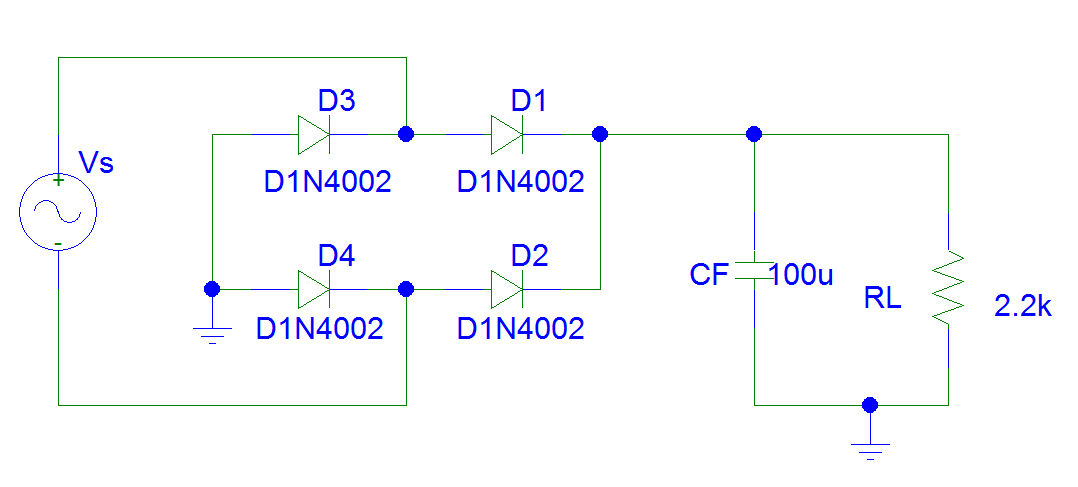
\includegraphics[width=\textwidth]{rekt_cap}
\caption{Full-wave rectifier with a capacitor filter.}
\label{fig:cap}
\end{subfigure}
\qquad
\begin{subfigure}[b]{0.45\textwidth}
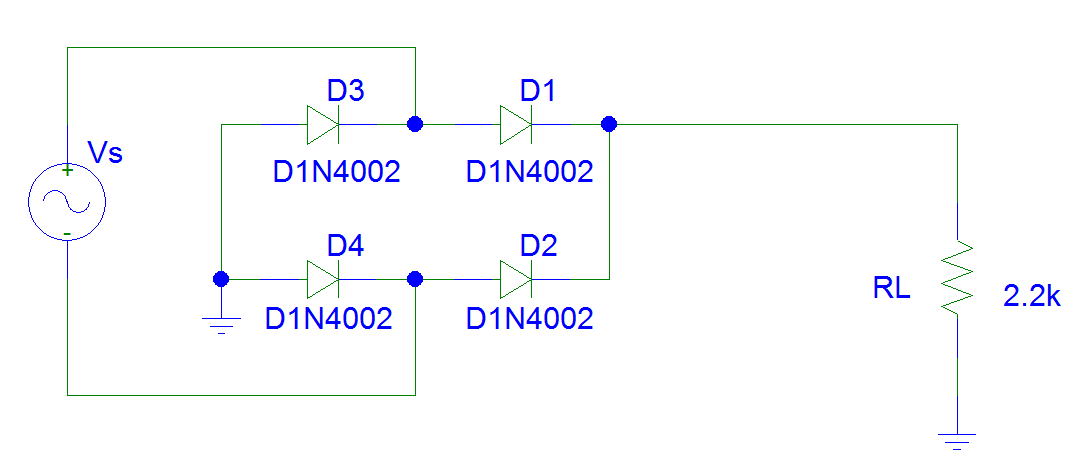
\includegraphics[width=\textwidth]{rekt_nocap}
\caption{Full-wave rectifier without a capacitor filter.}
\label{fig:nocap}
\end{subfigure}
\caption{Schematics.}
\label{fig:sch}
\end{figure}

To predict the output of the rectifier circuit, formulas from the lecture notes were used \citep{lecture}. The value for the input voltage $V_{in}$\footnote{Unless explicitly stated otherwise, all AC voltage values are peak-to-peak.} was taken to be equal to the actual output of the transformer used during testing (see Section~\ref{sec:imp}). The output voltage of a rectifier without a capacitor filter was calculated in Equation~\ref{eq:nocap}, and the voltage ripple and DC voltage output of the rectifier with a smoothing capacitor---in Equations \ref{eq:cap} and \ref{eq:capdc} respectively.
\begin{align}
\begin{split}
V_{out}&=V_{in}-2\times0.7\\
&=18.8-1.4\\
&=17.4\mathrm{V}
\label{eq:nocap}
\end{split}
\end{align}

Note that in the above case, in the absence of the smoothing capacitor, $V_r=V_{out}$. The addition of a capacitor has no effect on the output peak voltage, but decreases ripple.
\begin{align}
\begin{split}
  \begin{cases}
  V_{r}=\frac{V_{DC}}{2f R_L C}\\
  V_{DC}=V_{out}-\frac{1}{2}V_r
  \end{cases}
  \Leftrightarrow
  V_{r}&=\frac{2V_{out}}{4fR_LC+1}\\
  &=\frac{2\times17.4}{4\times50\times2.2\times10^{3}\times10^{-4}+1}\\
  &=0.773\mathrm{V}
\label{eq:cap}
\end{split}
\end{align}
\begin{align}
  \begin{split}
    V_{DC}&=V_{out}-\frac{1}{2}V_r\\
    &=17.4-\frac{0.773}{2}\\
    &=17.01\mathrm{V}
  \end{split}
  \label{eq:capdc}
\end{align}

\section{Simulation}
\label{sec:sim}
A series of PSPICE simulations were conducted to test the validity of the theoretical analysis. The results are recorded in Table~\ref{tab:sim}, and the input against output waveform graph of a full-bridge rectifier (Figure~\ref{fig:cap}) is shown in Figure~\ref{fig:norm}.
\begin{table}[h!]
\centering
\caption{Simulation results.}  
\begin{tabular}{|l|r|r|}
\hline
&$V_{out}$&$V_R$\\ \hline
Single resistor&$17.34\pm0.02\mathrm{V}$&$0.632\pm0.011\mathrm{V}$\\ \hline
Double resistors&$17.332\mathrm{V}$&$1.229\mathrm{V}$\\ \hline
\end{tabular}
\label{tab:sim}
\end{table}

When a second resistor of equivalent resistance was connected in parallel with the load resistor, the result in the PSPICE simulation was a doubling in the magnitude of the ripple voltage. This is to be expected as the result of placing two equivalent resistors in parallel is that the net resistance is halved. (Equation~\ref{eq:res}). Consequently the $RC$ constant halved---that is the capacitor was able to discharge faster---and as a result the voltage ripple was doubled (Figure~\ref{fig:res}). This behaviour is described in Equation~\ref{eq:vrpp}, which shows that peak to peak ripple voltage ($V_r$) is inversely proportional to $RC$.
\begin{align}
\begin{split}
 R_{total}&=\frac{1}{\frac{1}{R}+\frac{1}{R}}\\
&=\frac{R}{2}
\end{split}
\label{eq:res}
\end{align}
\begin{align}
\begin{split}
V_{r}=\frac{V_{DC}}{2f RC}
\end{split}
\label{eq:vrpp}
\end{align}
\begin{figure}[h!]
\centering
\begin{subfigure}[b]{0.65\textwidth}
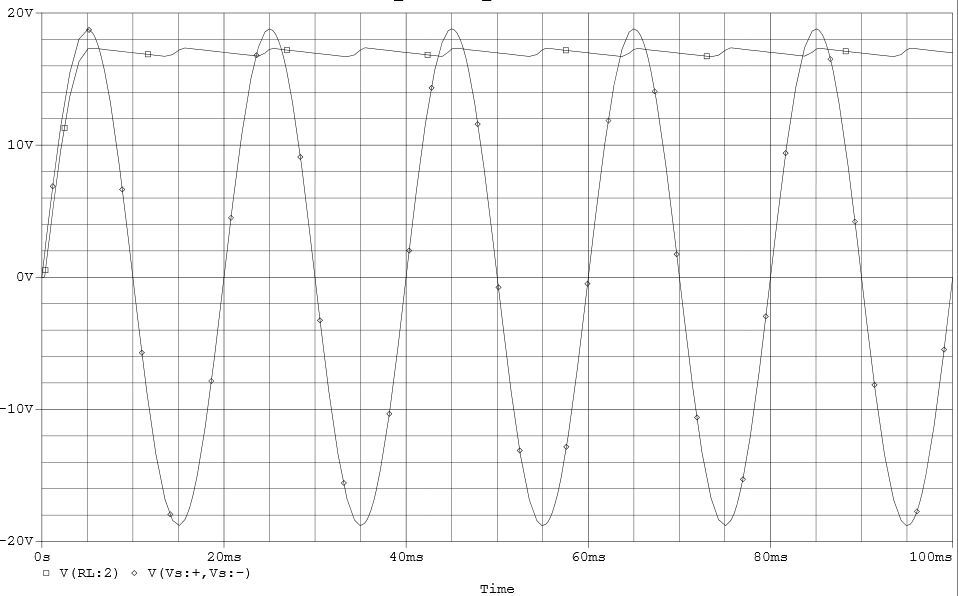
\includegraphics[width=\textwidth]{out_norm}
\caption{Normal rectifier with a capacitor.}
\label{fig:norm}
\end{subfigure}
\qquad
\begin{subfigure}[b]{0.65\textwidth}
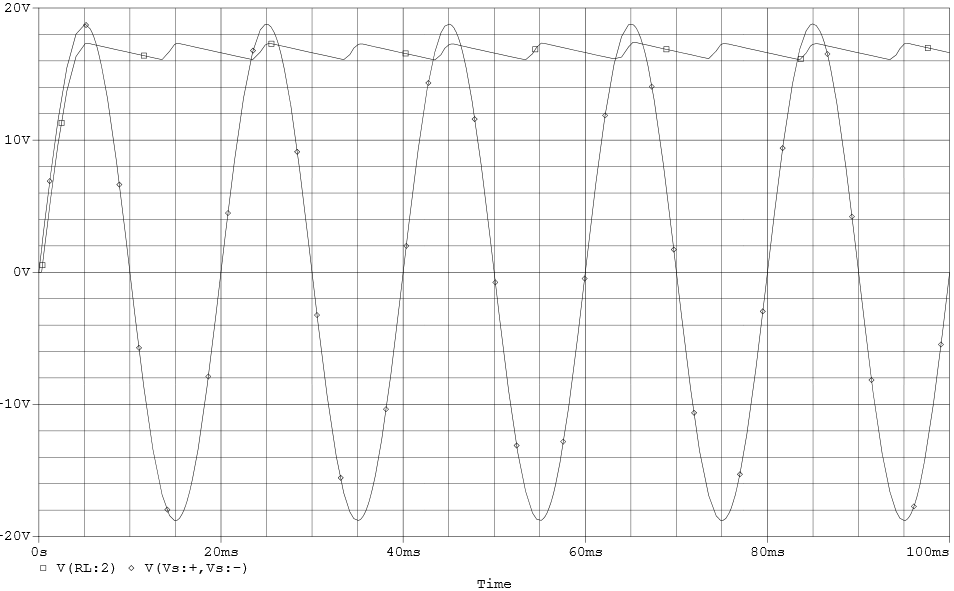
\includegraphics[width=\textwidth]{out_res}
\caption{Rectifier with two parallel load resistors.}
\label{fig:res}
\end{subfigure}
\caption{Simulation results.}
\label{fig:sim}
\end{figure}

PSPICE was also used to predict the outcome in the case of a faulty diode. To do this two scenarios were simulated, one in which the diode acts as an open circuit and one in which the diode acts as a short circuit. For these simulations, diode 4 (D4) was varied (Figure~\ref{fig:cap}).

In the short circuit scenario, the rectifier functioned as a half wave rectifier that only permitted the positive half-cycle to flow across the load resistor (Figure~\ref{fig:pos}). This is because during the negative cycle, a short circuit was created between the negative and positive outputs of the source. That is, as D4 no longer blocked current, current from the negative terminal could flow through D3 and back to the source without passing over the load resistor. During the positive half cycle there is not short a circuit as D3 acts as an open circuit with respect to the path of current.

In the open circuit scenario, the circuit functioned as a half wave rectifier that permitted only the negative cycle (Figure~\ref{fig:neg}). This is because during the positive cycle an open circuit between ground and the negative source terminal is produced, preventing current from flowing across the load resistor. However, when functioning normally D4 acts as an open circuit with the respect to the path of current during the negative half-cycle and therefore the negative half-cycle is unaffected.

If the same simulations are applied to the other diodes, a faulty D1 has the same effect as D4. D3 and D2 however block the positive cycle when acting as an open circuit and the negative cycle when acting as a short circuit.
\begin{figure}[h!]
\centering
\begin{subfigure}[b]{0.65\textwidth}
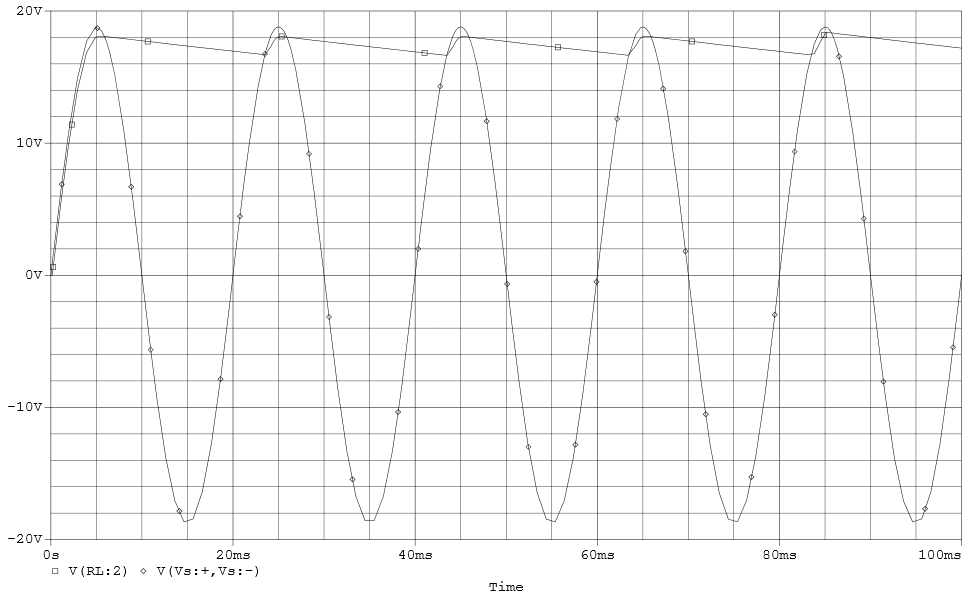
\includegraphics[width=\textwidth]{out_pos}
\caption{Positive half-cycle only.}
\label{fig:pos}
\end{subfigure}
\qquad
\begin{subfigure}[b]{0.65\textwidth}
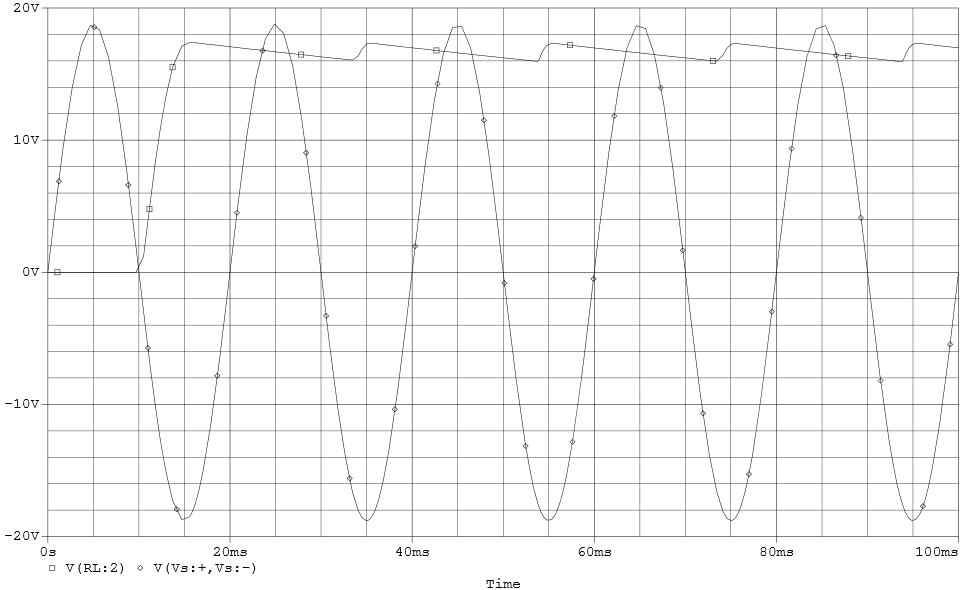
\includegraphics[width=\textwidth]{out_neg}
\caption{Negative half-cycle only.}
\label{fig:neg}
\end{subfigure}
\caption{Fault simulation results.}
\label{fig:fault}
\end{figure}

\section{Implementation}
\label{sec:imp}
The rectifier circuit was first built according to Figure~\ref{fig:nocap}, then modified with a smoothing capacitor (Figure~\ref{fig:cap}), and finally fitted with a voltage regulator, as shown in Figure~\ref{fig:reg}. The completed circuit, with the components labeled, soldered on a PCB can be seen in Figure~\ref{fig:pcb}.
\begin{figure}[h!]
\centering
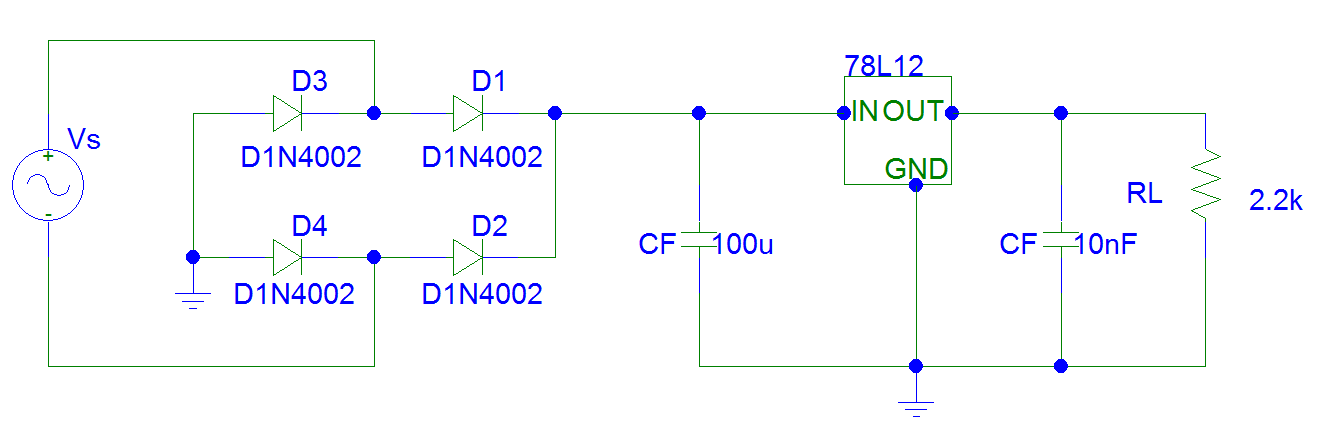
\includegraphics[width=0.6\textwidth]{rekt_reg}
\caption{Rectifier with a voltage regulator.}
\label{fig:reg}
\end{figure}
\begin{figure}[h!]
\centering
\begin{subfigure}[b]{0.45\textwidth}
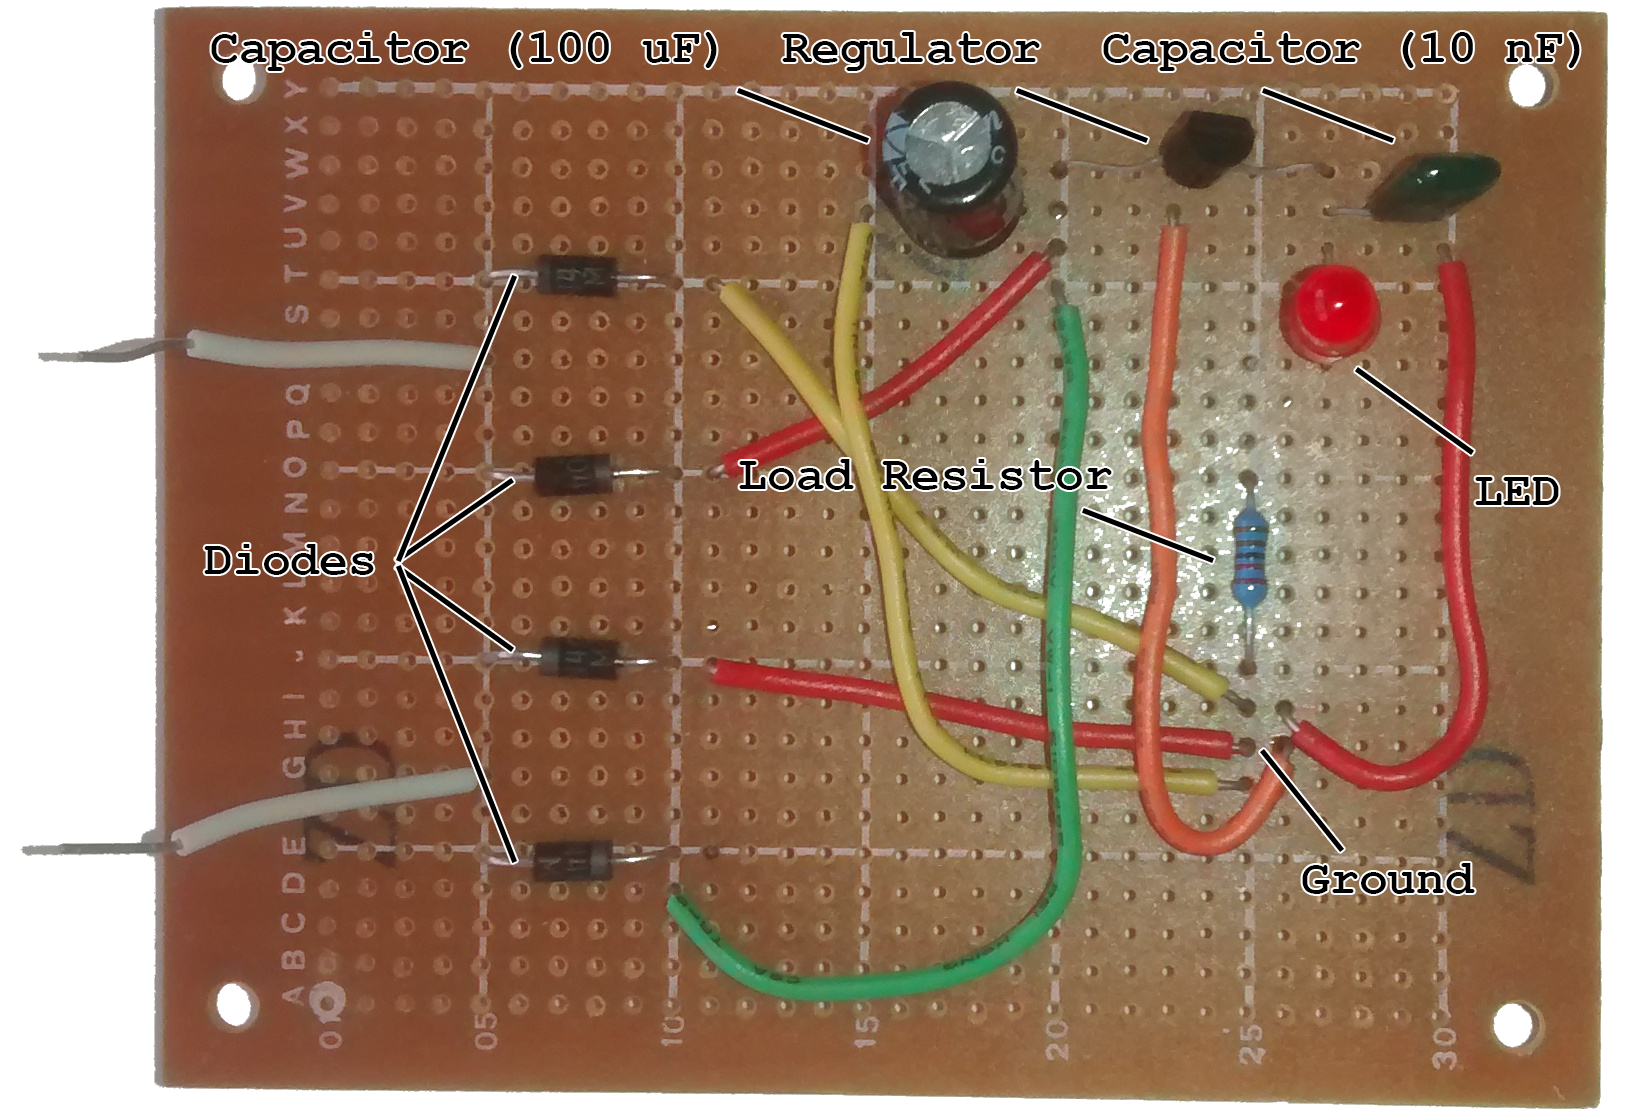
\includegraphics[width=\textwidth]{pcb_front}
\caption{Front.}
\label{fig:front}
\end{subfigure}
\qquad
\begin{subfigure}[b]{0.41\textwidth}
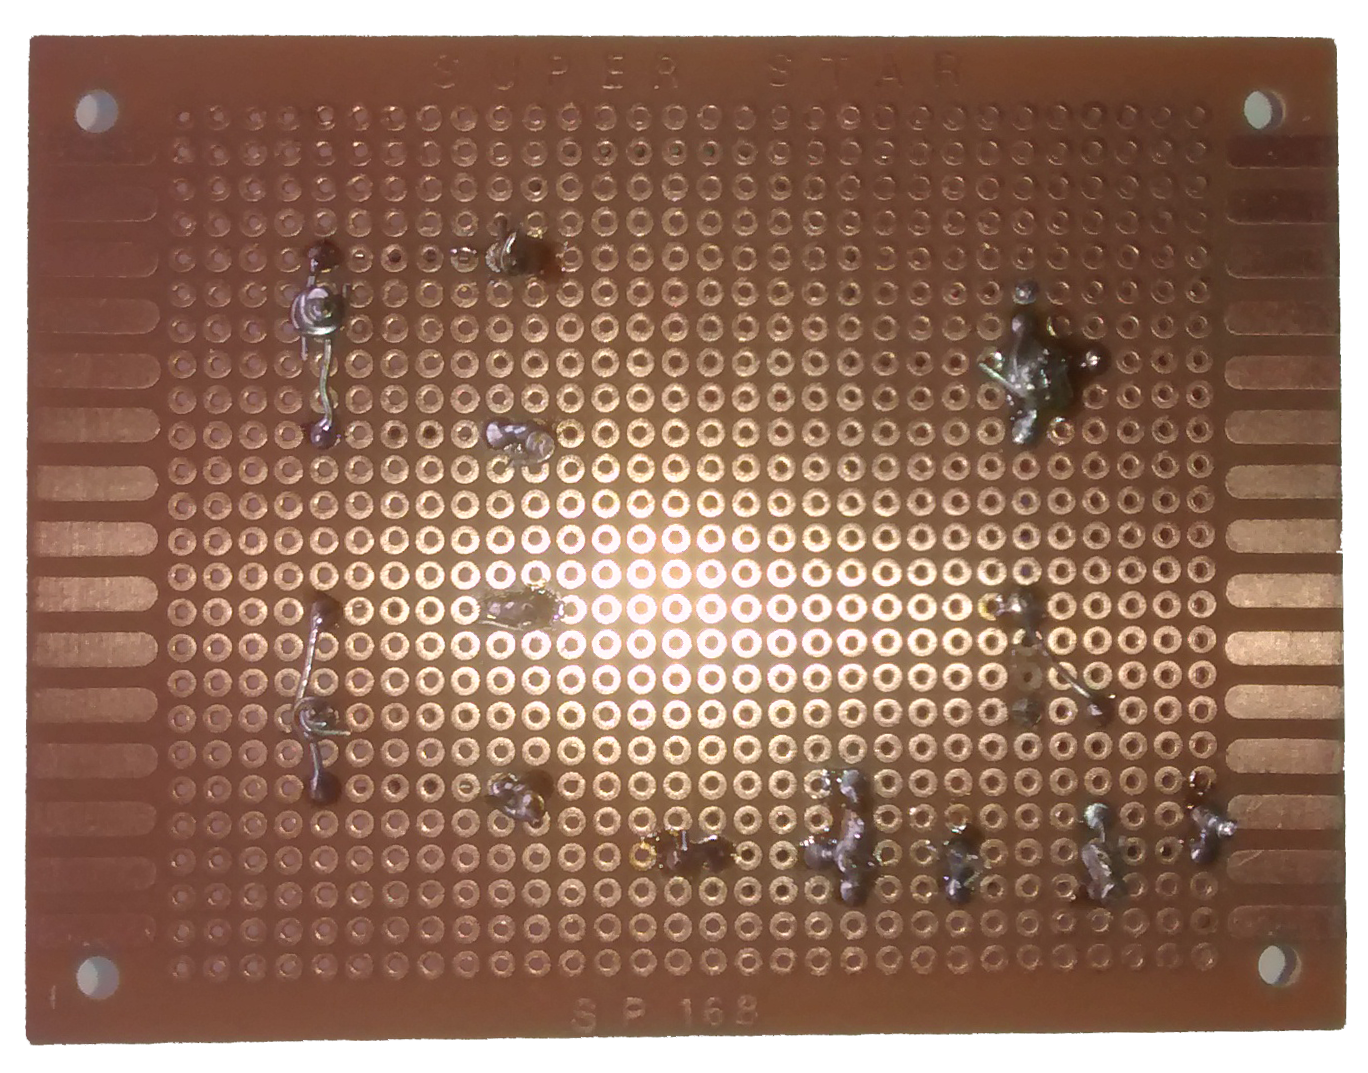
\includegraphics[width=\textwidth]{pcb_back}
\caption{Back.}
\label{fig:back}
\end{subfigure}
\caption{Finished circuit.}
\label{fig:pcb}
\end{figure}

The measurements taken from the three versions of the circuit are presented in Table~\ref{tab:imp}.
\begin{table}[h!]
\centering
\caption{Measurements.}  
\begin{tabular}{|l|r|r|r|r|r|r|}
\hline
&$V_{in}(\mathrm{V})$&$V_{out}(\mathrm{V})$&$V_{DC}(\mathrm{V})$&$V_{r}(\mathrm{V})$&$R_{L}(\mathrm{\Omega})$&$f_{out}(\mathrm{Hz})$\\ \hline
no capacitor&$18.8$&$17.4$&--&17.4&$2197$&$100$\\ \hline
with capacitor&$18.8$&$17.4$&16.9&0.7&$2197$&$100$\\ \hline
with regulator&$18.8$&\multicolumn{2}{|c|}{12.1}&0.02&$2197$&$100$\\ \hline
\end{tabular}
\label{tab:imp}
\end{table}

\section{Discussion}
\label{sec:dis}
As per Table~\ref{tab:dis}, there were significant differences between simulated, measured and predicted ripple values. There is a difference of approximately $0.07\mathrm{V}$ between the measured ripple voltage and both the simulated and predicted values. What is notable is that there is roughly a $0.14\mathrm{V}$ difference between the simulated value and the predicted value that was calculated using the approximation formulas (Equation~\ref{eq:vrpp}). Despite being an approximation, the predicted value was expected to be much closer to the simulated value. In the approximation formula the assumption is made that once the AC voltage reaches its maximum, the signal is switched off and the capacitor is left to discharge until the AC voltage reaches its next maximum.
\begin{table}[h!]
\centering
\caption{Comparsion of results.}  
\begin{tabular}{|l|r|r|r|r|r|r|r|r|r|r|}
\hline
&\multicolumn{3}{|c|}{$V_{out}(\mathrm{V})$}&\multicolumn{3}{|c|}{$V_{DC}(\mathrm{V})$}&\multicolumn{3}{|c|}{$V_{r}(\mathrm{V})$}\\ \hline
&pred.&sim.&meas.&pred.&sim.&meas.&pred.&sim.&meas.\\ \hline
no capacitor&$17.4$&$17.34$&$17.4$&--&--&--&$17.4$&$17.32$&17.4\\ \hline
with capacitor&$17.4$&$17.32$&$17.4$&17.01&$17.02$&16.92&$0.77$&$0.63$&0.7\\ \hline
with regulator&$12.0$&--&$12.1$&12.0&--&12.1&$0$&--&0.02\\ \hline
\end{tabular}
\label{tab:dis}
\end{table}
 
This however, is not the case as the AC voltage decreases as a sinusoidal function---as AC voltage is sinusoidal---to zero. Therefore, the capacitor equation (Equation~\ref{eq:nat}) for a natural response cannot be used directly to calculate the drop in voltage of the capacitor. Instead it must be viewed as a series of step responses each with a new DC source voltage after time $\mathrm{d}t$. The source voltage at time t is given by the magnitude of the voltage due to the AC wave at that time. This can be thought of as the voltage available for discharge not being the voltage of the capacitor with respect to ground, but delta V between the voltage of the capacitor and the voltage due to the AC source. Consequently the ripple voltage magnitude will be smaller than the predicted value as delta V between capacitor and source is never as large as initial voltage of the capacitor used in the approximation equation.
 
The $0.07\mathrm{V}$ difference between the simulated result and the measured result is also significant. However, there were several error sources within the experiment that may have contributed to this disparity. Firstly, the capacitance of electrolytic capacitors can have uncertainties of 20\% \citetext{Electronics Tutorials}. The magnitude of this uncertainty comes from a number of different sources such as temperature and variation in frequency of the input signal. Therefore, for a $100\mathrm{\mu F}$ capacitor, $\sigma_C=20\mathrm{\mu F}$. There is also the uncertainty in the resistance of the resistor which according to the colour bands on the resistor is 1\%, thus  $\sigma_R=22\mathrm{\Omega}$. These errors were then propagated for the capacitor voltage natural response formula (Equation~\ref{eq:nat}) using the following error propagation formulas \citetext{Rochester Institute of Technology}.
\begin{align}
V(t)=V_0e^{-\frac{t}{RC}}
\label{eq:nat}
\end{align}

The propagated uncertainty was found to be $0.156\mathrm{V}$. The difference between the measured and mean simulated ripple value was $0.068\mathrm{V}$, with an uncertainty of $0.0156\mathrm{V}$---the uncertainty in the simulated values was small and consequently did not change the error significantly. Therefore, the measured ripple voltage was within $0.44\sigma$ of the mean simulated ripple voltage. Thus the measured value agreed with the simulated value to a considerable degree considering the high uncertainty.
 
Other sources of error such as fluctuations in the output signal measured by the oscilloscope and resistance in the wires of the circuit would also have contributed to the error. However, these would have been relatively small and the measured result was already found to agree with the simulated result to an acceptable degree.

In the regulated version of the circuit, the output voltage was limited to $12.1\mathrm{V}$ with a negligible ripple of $20\mathrm{mV}$. Thus, the target ($12\mathrm{V}$ DC output with 10\% tolerance) was successfully achieved. Although the predicted output was $12\mathrm{V}$, the difference of $0.1\mathrm{V}$ was caused by the voltage output tolerance of the 78L12 regulator, which, according to the datasheet \citetext{Texas Instruments} can vary from $11.5\mathrm{V}$ to $12.5\mathrm{V}$ depending on the input voltage and current.

\section{Conclusion}
\label{sec:con}
The full-wave diode bridge power rectifier circuit was built and analysed, the output values were compared with theoretical predictions and PSPICE simulation results. Due to parameter deviations in the circuit components and inaccuracy of the approximation formulas, the results did not match perfectly, but the errors were analysed using uncertainty propagation and found plausible.

The two methods for predicting the output of the rectifier circuit were shown to be acceptably accurate. Using higher grade components and measuring equipment would have reduced the error.

Despite functioning as expected, the circuit itself was not planned to incorporate changes like the addition of components such as the regulator and the extra capacitor. Consequently, it was difficult to connect some components to the required nodes and as a result extra wires had to be used to perform these connections. Furthermore, some already soldered connections had to be cut and then resoldered elsewhere. This made the circuit difficult to understand and also more time consuming to construct. In future the circuit should be planned before hand such that it is constructed in a manner that is easy to comprehend.
\bibliography{report}
\section*{Reflection}
This lab provided important theoretical knowledge as well as the skills required to implement and test it. I learnt a lot considering the amount of time spent in the lab. The most significant thing I learnt was the importance of projecting and planning in the physical implementation of a circuit.
\end{document}
